\chapter{Desarrollo del Proyecto} % (fold)
\label{cha:desarrollo}

Ya que para el desarrollo del proyecto se usará programación extrema,
se va a definir el proceso de desarrollo general que se usará en este proyecto
de grado.\\

  % \section{Proceso de Desarrollo}
  % \label{sec:proceso_de_desarrollo}

  XP propone un proceso iterativo e incremental, El proyecto es dividido en pequeños “mini-proyectos”, los cuales terminan con un release\footnote{\emph{Release} es una versión del producto que se libera al final de un ciclo de desarrollo de software, un release contiene requerimientos implementados, tal vez no acabados en un  100\% pero funcional de tal forma el cliente es capaz de ofrecer feedback del producto.} o lanzamiento.\\

En un proyecto que sigue la metodología XP los releases son frecuentes, esto para recibir feedback más seguido. Los releases son negociados en un Planning Game, donde los clientes definen qué se va a implementar en el release y los desarrolladores especifican el tiempo que necesitan para desarrollar las características deseadas.\\

\begin{figure}[H]
  \caption{Diagrama del proceso XP}
  \label{fig:xp_diagram}
  \begin{center}
    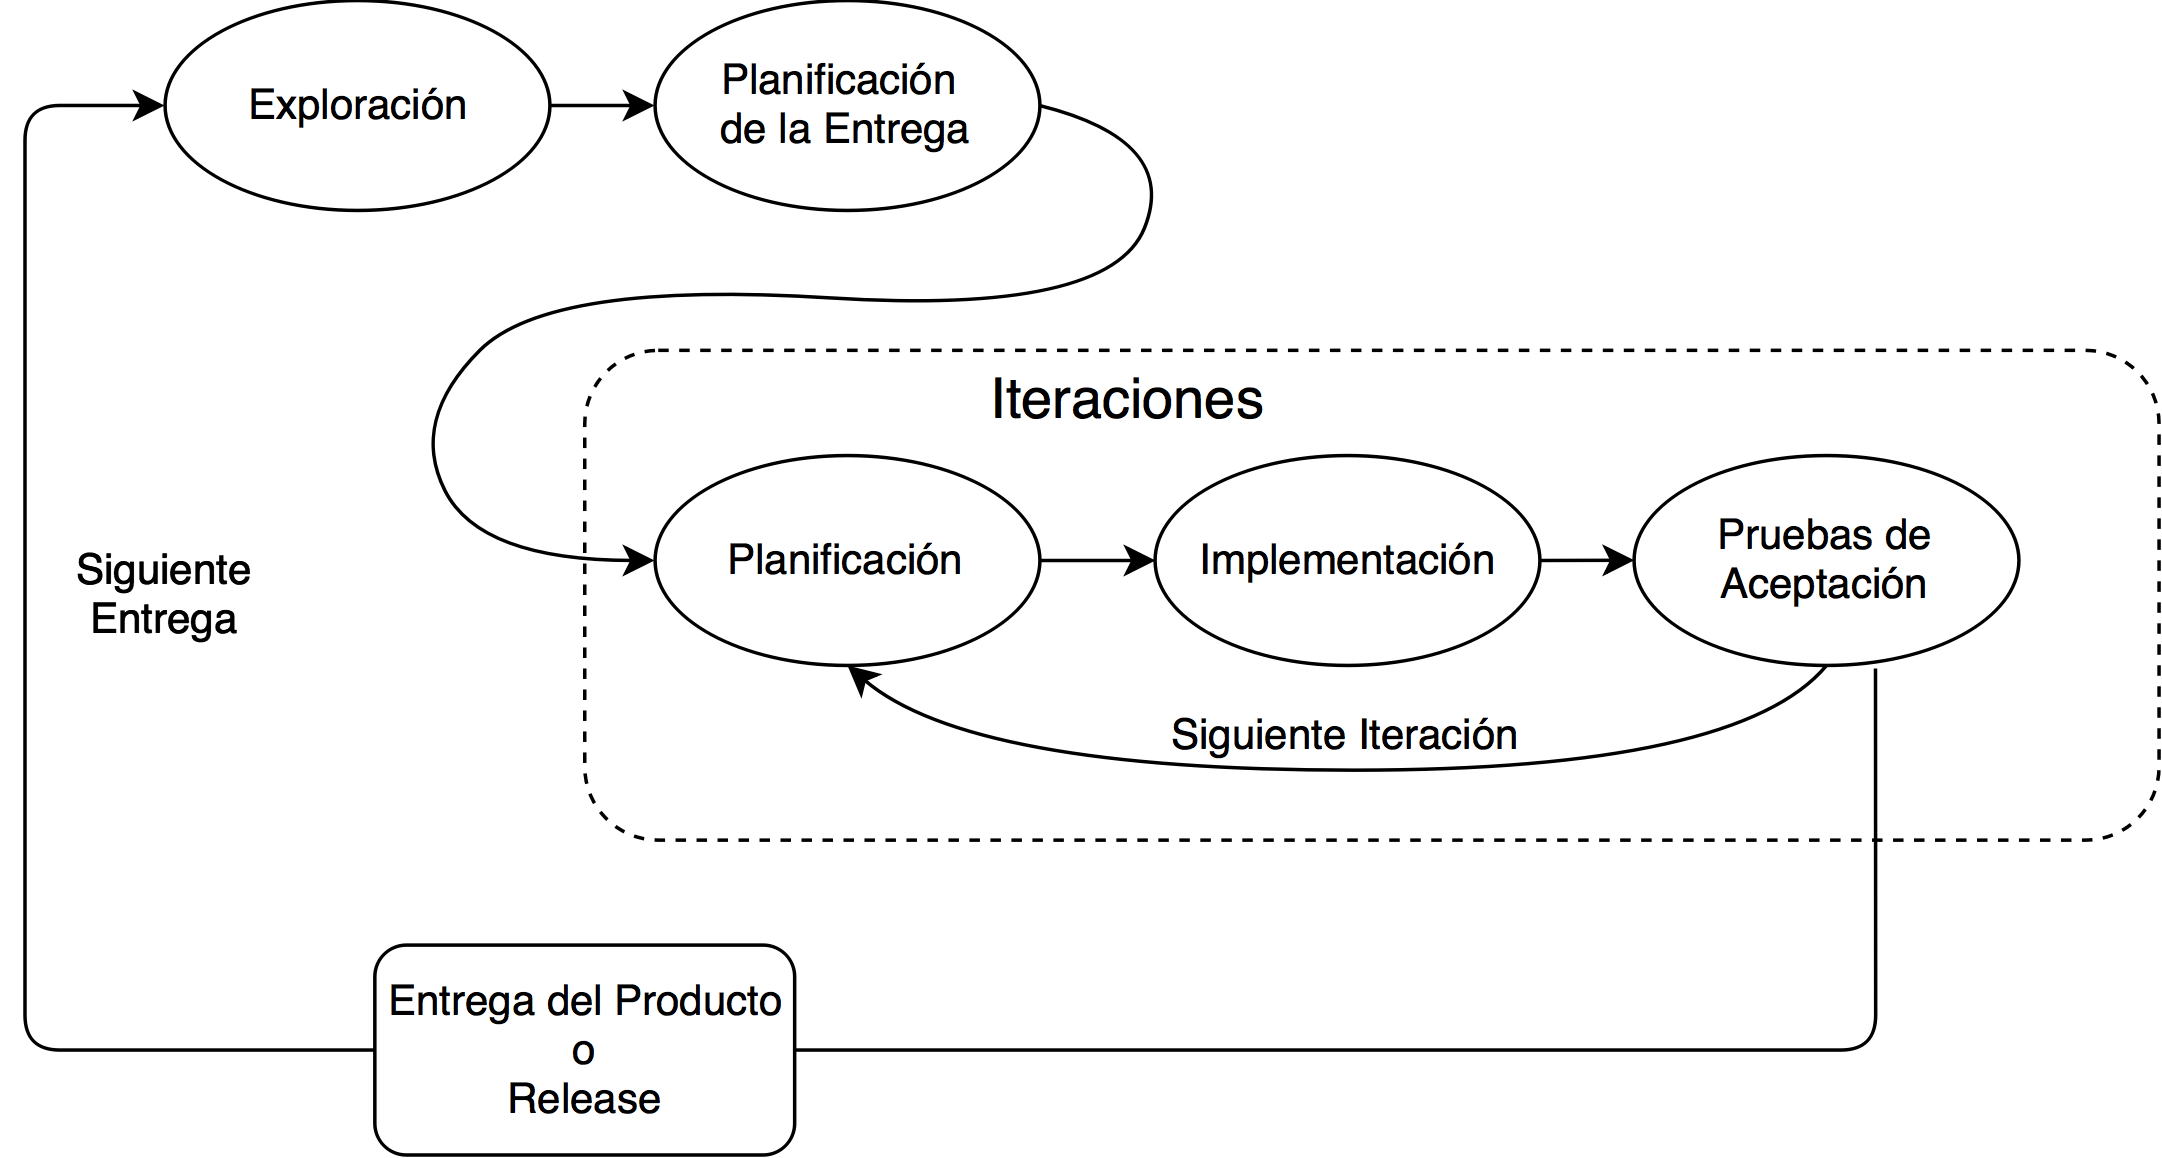
\includegraphics[width=1\textwidth]{xp_diagram}
  \end{center}
  \caption*{Fuente: Elaboración propia}
\end{figure}

En la figura \ref{fig:xp_diagram} se puede apreciar el proceso de desarrollo de la metodología XP, la cual se explicará a continuación.\\

  \section{Planning Game}
  \label{sec:planning_game}

  La fase del planning game consiste de 3 etapas: exploración, planeaci\'on y direcci\'on.\\

  Durante la fase de la \textbf{exploración} los clientes definen lo que desean que tenga el sistema y los desarrolladores estiman el tiempo necesario que necesitan para realizar esas tareas.\\

  Durante la \textbf{planeación} se negocia y se decide cuales de todas las características que los clientes quieren pueden llegar a realizarse en el tiempo dise~ado para una iteración.\\

  Después de la planeación sigue la fase de \textbf{dirección}, durante la cual se desarrolla y actualiza (cuando sea necesario) la planeación ya negociada según lo que se vaya aprendiendo a medida que avanza el desarrollo del proyecto.\\

    \subsection{Exploración}
    \label{sub:exploracion}
      Durante esta etapa el cliente escribe las tarjetas de historias de usuario, estas historias definen lo que el cliente quiere que el sistema haga, en otras palabras representan las características que el sistema debería tener implementado.\\

      Una vez que estas tarjetas están escritas, el equipo de desarrollo debe asignarles una estimación en términos del tiempo necesitado para el desarrollo y el riesgo para el producto que pueden llegar a tener las características detalladas en las historias del usuario.\\

      Las historias del usuario se las crea para propósitos de planeación y estimación de tiempo y esfuerzo que cada característica va a necesitar, los detalles se crean y dividen posteriormente cuando las historias están por ser implementadas en las “tareas de ingeniería”.\\
    % end exploracion

    \subsection{Planeación}
    \label{sub:planeacion}

      Cuando se tienen las historias del usuario junto con las estimaciones de los desarrolladores, se está listo para una “negociación de aceptación” donde un “calendario de entregas”  es negociado y donde se aceptan qué historias se van a desarrollar primero en cuanto tiempo se van a entregar resultados.\\

    % end planeacion

    \subsection{Dirección o Steering}
    \label{sub:steering}

    Esta fase es básicamente comprende el resto del desarrollo del producto hasta que es liberado al mercado o el proyecto es cancelado.\\

    Esta fase consiste en 4 ``movimientos'':

    \begin{description}
      \item[Iteración:] Es durante la iteración cuando se desarrolla el producto, el tiempo que se utiliza para esta fase es de generalmente de una o 2 semanas, dependiendo de la naturaleza del proyecto.

      \item[Recuperación:] Si durante el desarrollo no se completan las características a desarrollar en el tiempo establecido, es durante la recuperación que se re-negocia con el cliente si quiere cambiar la fecha de entrega del release o modificar el alcance del desarrollo (menos historias de usuario).

      \item[Nuevas Historias:] El cliente tiene el derecho de aumentar historias de usuario, las cuales se tienen que estimar y negociar si serán parte del actual desarrollo, en tal caso se tiene que renegociar las fechas de entrega.

      \item[Re-estimación:] Si durante el desarrollo el equipo considera que el plan ya no es correcto, todas las historias que faltan hacer se tienen que re-estimar y el plan se tiene que re-negociar con el cliente.
    \end{description}

  % end planning_game

    \section{Iteration Planning Game}
    \label{sec:iteracion}

      % \subsubsection{Iteración}
      % \label{subs:iteracion}

      La fase de Iteración en XP se lo denomina como Iteration Planning Game, esta al igual que  el release planning game consiste en las fases de: Exploración, Planning e Implementaci\'on. Steering.\\

      Hay que tomar en cuenta que la planeación de una iteración en particular es desarrollada al inicio de cada interacción, no se planifican iteraciones por adelantado.\\

      Generalmente cada 3 iteraciones se actualiza el Calendario de Entregas “committed schedule” para reflejar los logros alcanzados por el equipo de desarrollo y el estado del proyecto, también sirve para identificar posibles riesgos.\\

      \subsection{Exploración}
      \label{sub:exploracion}

      Durante esta fase el cliente escoge las historias de usuario que serán implementadas en la presente iteración, generalmente se escogen las que aportan más valor al producto o tienen más relevancia en la lógica de negocio del cliente, asi como tambien cualquier historia que no se acabó en una iteración anterior.\\

      Los desarrolladores dividen las historias en Tareas de Ingeniería, las cuales son más pequeñas que las historias, si se encuentra que una Tarea es casi tan grande como una historia es porque es una historia y debería ser dividida en Tareas. Una tarea puede estar relacionada a 2 o mas historias o no estar relacionada con ninguna historia. Dentro de la metodología XP es una buena práctica el escribir las tareas en las  “Index Cards”, similares a las historias, esto debido a que estas tarjetas son fáciles de manipular durante la fase de planeación.\\

      % end exploracion

      \subsection{Planeación}
      \label{sub:planeacion}

      Durante esta fase un desarrollador acepta la responsabilidad de implementar una Tarea de acuerdo de su experiencia personal en el área y tecnologías que se usarán en el desarrollo. El desarrollador debe estimar el tiempo necesitado para completar la tarea en un \emph{Ideal Engineering Time} Tiempo de Ingenieria Ideal, siempre hay que considerar que la tarea se deriva de la Historia de usuario que es escogido para la iteración actual, una regla de XP consiste en que no se debe realizar trabajo el cual no se va necesitar ahora, \textbf{YAGNI}\footnote{You aren't gonna need it. En espa\~nol, Tu no lo vas a necesitar \'o No vas a necesitarlo.}.\\

      La Tarea combinada con el nombre del desarrollador responsable, la estimación asignada son parte del \emph{Iteration Schedule} \'o \emph{Plan de la Iteración}, con el cual el equipo de desarrollo es capaz de determinar si la iteración está \emph{floja} o \emph{cargada}, si está \emph{floja} se pueden añadir otras historias a la iteración o si está \emph{cargada} es necesario dividir historias.\\
      Finalmente cuando la carga de trabajo de la iteración está balanceada se procede con la siguiente fase, la \emph{Implementación} de las tareas.


      % end planeacion

      \subsection{Implementación}
      \label{sub:implementacion}

      % dentro de la Implementación una Tarea de desarrollar.
      Dentro de lo que es el ciclo de desarrollo de software, \textbf{XP} define el siguiente procedimiento:

      \begin{itemize}
        \item Analizar lo que hay que hacer, esto envuelve lo que es analizar las Tarjetas de Ingeniería y/o las historias de usuario. %, de ser necesario se realiza una sesión CRC.
        \item Escribir Pruebas Unitarias, son bastante útiles para determinar cuando la tarea está completada.
        \item Implementar el código suficiente para lograr que las pruebas unitarias pasen exitosamente.
        \item Simplificar el código si es necesario (Refactor Mercilessly).
        \item Integrar los cambios continuamente (Continuous Integration).
      \end{itemize}
      % end implementacion

      \subsection{Registrar el Avance}
      \label{sub:registrar_avance}
      XP define un rol en específico que se encarga de medir el progreso, el Tracker.

      \subsection{Verificación}
      \label{sub:verificacion}
      Cada historia lleva asociado test funcionales, que están diseñados para verificar que los criterios de aceptación de cada historia están implementados. \\
      Si durante esta fase las pruebas fallan, la historia de usuario relacionada se marca para volver a trabajar en ella en la siguiente iteración.\\


      % end iteracion

    % end steering



  % end proceso_de_desarrollo

  \section{Implementación del proyecto}
  \label{sec:implementacion}

  Siguiendo la metodología XP, el presente proyecto de grado debe empezar por la primera etapa del Planning Game.\\



  Exploración - Entrega y estimación de las historias de usuario

    \subsection{Historias de Usuario}
    \label{sub:historias_de_usuario}

      % % user_story_01
% % \begin{table}[!ht]
% \begin{table}[H]
%   \begin{center}
%     \begin{tabular}{ L{3cm}  L{8cm} }
%       \toprule
%         \textbf{Historia} US01 &
%         % \textbf{Esfuerzo} 5 puntos \\
%         \makebox[6cm][r]{\textbf{Esfuerzo} 8 puntos} \\
%         % \makebox[4cm][r]{\textbf{Estimación} 3 días} \\
%
%       \midrule
%       \multirow{3}{*}{\textbf{Descripción}}
%         & Yo como visitante\\
%         & Deseo registrarme en el sistema\\
%         & Para poder acceder al sistema\\
%       \midrule
%         \multirow{3}{3cm}{\textbf{Criterios de Aceptación}}
%         & Quiero ver fácilmente que no estoy registrado\\
%         & Quiero que el registro solamente me pida un nombre de usuario y un password\\
%         & Quiero ver que al estar registrado pueda acceder a los lugares\\
%       \bottomrule
%     \end{tabular}
%     \caption{Historia de Usuario - US01}
%     \label{tab:user_story_01}
%   \end{center}
% \end{table}

% user_story_02

% user_story_03

\begin{table}[H]
  \begin{center}
    \begin{tabular}{ L{3cm}  L{8cm} }
      \toprule
        \textbf{Código:} & US01 \\
        \textbf{Prioridad:} & Alta \\
        \textbf{Riesgo:} & Alta \\

        % \addlinespace
      \midrule
        \multirow{3}{*}{\textbf{Descripción:}}
        & Yo como visitante\\
        & Deseo ver una lista de lugares \\
        % & Deseo ingresar el nombre de un lugar\\
        & Para encontrar el lugar al que deseo ir\\
        \addlinespace
      % \midrule
        \multirow{3}{3cm}{\textbf{Criterios de Aceptación:}}
        & Quiero tener los lugares en una base de datos \\
        & Quiero ver una lista de lugares\\
        & Quiero filtrar la lista de lugares por el nombre o parte de este\\
        % & Quiero encontrar un lugar
        % & Quiero encontrar un lugar y poder ver su información\\
      \bottomrule
    \end{tabular}
    \caption{Historia de Usuario - US01}
    \label{tab:user_story_01}
  \end{center}
\end{table}

\begin{table}[H]
  \begin{center}
    \begin{tabular}{ L{3cm}  L{8cm} }
      \toprule
        \textbf{Historia} US02 &
        % \textbf{Esfuerzo} 5 puntos \\
        \makebox[6cm][r]{\textbf{Esfuerzo} 8 puntos} \\
        % \makebox[4cm][r]{\textbf{Estimación} 3 días} \\

      \midrule
        \multirow{3}{*}{\textbf{Descripción}}
        & Yo como visitante\\
        & Deseo ver la información de un lugar\\
        & Para decidir si es el lugar que estoy buscando\\
      \midrule
        \multirow{3}{3cm}{\textbf{Criterios de Aceptación}}
        & Quiero leer una descripción del lugar\\
        & Quiero ver un teléfono asociado al lugar\\
        & Quiero ver en qué piso se encuentra el lugar\\
      \bottomrule
    \end{tabular}
    \caption{Historia de Usuario - US02}
    \label{tab:user_story_02}
  \end{center}
\end{table}



% user_story_03

\begin{table}[H]
  \begin{center}
    \begin{tabular}{ L{3cm}  L{8cm} }
      \toprule
        \textbf{Historia} US03 &
        % \textbf{Esfuerzo} 5 puntos \\
        \makebox[6cm][r]{\textbf{Esfuerzo} 8 puntos} \\
        % \makebox[4cm][r]{\textbf{Estimación} 3 días} \\

      \midrule
        \multirow{3}{*}{\textbf{Descripción}}
        & Yo como visitante\\
        & Deseo ver el lugar en un mapa\\
        & Para saber en que parte del campus se encuentra el lugar\\
      \midrule
        \multirow{3}{3cm}{\textbf{Criterios de Aceptación}}
        & Deseo ver sobre un mapa un punto del lugar buscado a donde quiero ir\\
        & Quiero ver un marcador sobre el lugar que estoy buscando con alguna información para asegurarme que es a donde quiero ir\\

      \bottomrule
    \end{tabular}
    \caption{Historia de Usuario - US03}
    \label{tab:user_story_03}
  \end{center}
\end{table}


% user_story_04

\begin{table}[H]
  \begin{center}
    \begin{tabular}{ L{3cm}  L{8cm} }
      \toprule
        \textbf{Historia} US04 &
        % \textbf{Esfuerzo} 5 puntos \\
        \makebox[6cm][r]{\textbf{Esfuerzo} 8 puntos} \\
        % \makebox[4cm][r]{\textbf{Estimación} 3 días} \\

      \midrule
        \multirow{3}{*}{\textbf{Descripción}}
        & Yo como visitante\\
        & Deseo ver una ruta sobre el mapa\\
        & Para encontrar el lugar de forma rapida\\
      \midrule
        \multirow{1}{3cm}{\textbf{Criterios de Aceptación}}
        & Deseo ver sobre un mapa un punto del lugar actual donde me encuentro\\

        & Deseo ver una línea roja que muestre la ruta más corta para llegar de mi ubicación al lugar donde quiero ir\\

      \bottomrule
    \end{tabular}
    \caption{Historia de Usuario - US04}
    \label{tab:user_story_04}
  \end{center}
\end{table}


% user_story_04

\begin{table}[H]
  \begin{center}
    \begin{tabular}{ L{3cm}  L{8cm} }
      \toprule
        \textbf{Historia} US05 &
        % \textbf{Esfuerzo} 5 puntos \\
        \makebox[6cm][r]{\textbf{Esfuerzo} 8 puntos} \\
        % \makebox[4cm][r]{\textbf{Estimación} 3 días} \\

      \midrule
        \multirow{3}{*}{\textbf{Descripción}}
        & Yo como visitante\\
        & Deseo registrarme\\
        & Para tener mas opciones dentro el sistema\\
      \midrule
        \multirow{3}{3cm}{\textbf{Criterios de Aceptación}}
        & Quiero ver un formulario donde me pueda registrar.\\
        & Una vez registrado quiero poder ingresar al sistema con mis credenciales.\\
        & Quiero ver tener la posibilidad de editar mis datos.\\
      \bottomrule
    \end{tabular}
    \caption{Historia de Usuario - US05}
    \label{tab:user_story_05}
  \end{center}
\end{table}



% user_story_05

\begin{table}[H]
  \begin{center}
    \begin{tabular}{ L{3cm}  L{8cm} }
      \toprule
        \textbf{Historia} US06 &
        % \textbf{Esfuerzo} 5 puntos \\
        \makebox[6cm][r]{\textbf{Esfuerzo} 8 puntos} \\
        % \makebox[4cm][r]{\textbf{Estimación} 3 días} \\

      \midrule
        \multirow{3}{*}{\textbf{Descripción}}
        & Yo como usuario registrado\\
        & Deseo añadir más lugares al sistema\\
        & Para mejorar los criterios de busqueda\\
      \midrule
        \multirow{3}{3cm}{\textbf{Criterios de Aceptación}}
        & Quiero que sea posible anadir un lugar si no lo encuentro en la lista de lugares\\
        & Quiero ver un formulario para poder ingresar los datos de un nuevo lugar.\\
        & Quiero pararme cerca o en el lugar que necesito añadir para geo-referenciarlo\\
        % & Al añadir un lugar necesito ingresar alguna descripción y/o teléfono si fuera necesario\\
      \bottomrule
    \end{tabular}
    \caption{Historia de Usuario - US06}
    \label{tab:user_story_06}
  \end{center}
\end{table}



% user_story_06

\begin{table}[H]
  \begin{center}
    \begin{tabular}{ L{3cm}  L{8cm} }
      \toprule
        \textbf{Historia} US07 &
        % \textbf{Esfuerzo} 5 puntos \\
        \makebox[6cm][r]{\textbf{Esfuerzo} 8 puntos} \\
        % \makebox[4cm][r]{\textbf{Estimación} 3 días} \\

      \midrule
        \multirow{3}{*}{\textbf{Descripción}}
        & Yo como usuario registrado\\
        & Deseo editar la información de un lugar\\
        & Para mejorar o corregir la información de ese lugar\\
      \midrule
        \multirow{3}{3cm}{\textbf{Criterios de Aceptación}}
        & Al entrar a la información de un lugar quiero ser el único que vea un icono para poder entrar a la edición de los datos\\
        & Quiero acceder a un formulario que muestre la información actual del lugar y poder editar la información mostrada\\

      \bottomrule
    \end{tabular}
    \caption{Historia de Usuario - US07}
    \label{tab:user_story_07}
  \end{center}
\end{table}

% user_story_07

\begin{table}[H]
  \begin{center}
    \begin{tabular}{ L{3cm}  L{8cm} }
      \toprule
        \textbf{Historia} US08 &
        % \textbf{Esfuerzo} 5 puntos \\
        \makebox[6cm][r]{\textbf{Esfuerzo} 8 puntos} \\
        % \makebox[4cm][r]{\textbf{Estimación} 3 días} \\

      \midrule
        \multirow{3}{*}{\textbf{Descripción}}
        & Yo como usuario administrador\\
        & Deseo administrar usuarios\\
        & Para anadir o remover usuarios del sistema\\
      \midrule
        \multirow{3}{3cm}{\textbf{Criterios de Aceptación}}
        & Quiero ver los usuarios que desean registrarse en el sistema\\
        & Quiero aceptar o rechazar solicitudes de registro\\
        & Quiero eliminar usuarios que no usen el sistema de forma adecuada.\\

      \bottomrule
    \end{tabular}
    \caption{Historia de Usuario - US08}
    \label{tab:user_story_08}
  \end{center}
\end{table}


% user_story_08

\begin{table}[H]
  \begin{center}
    \begin{tabular}{ L{3cm}  L{8cm} }
      \toprule
        \textbf{Historia} US09 &
        % \textbf{Esfuerzo} 5 puntos \\
        \makebox[6cm][r]{\textbf{Esfuerzo} 13 puntos} \\
        % \makebox[4cm][r]{\textbf{Estimación} 3 días} \\

      \midrule
        \multirow{3}{*}{\textbf{Descripción}}
        & Yo como usuario administrador\\
        & Deseo ver los lugares más visitados\\
        & Para obtener información y estadísticas de los lugares dentro del campus Universitario\\
      \midrule
        \multirow{3}{3cm}{\textbf{Criterios de Aceptación}}
        & Quiero apreciar de forma sencilla la cantidad de veces que los usuarios buscan un lugar\\
        & Quiero poder guardarla el reporte\\

      \bottomrule
    \end{tabular}
    \caption{Historia de Usuario - US09}
    \label{tab:user_story_09}
  \end{center}
\end{table}


    % end historias_de_usuario

    \subsection{Planeacion de Entregas}
    \label{sub:Planeacion de Entregas}

        A continuación el calendario de entregas del proyecto, el cual de acuerdo de las historias de usuario recogidas se estimó para unas 4 Iteraciones, y cada Iteración de 2 semanas.\\

        % \begin{table}[!ht]
%
% \end{table}
\begin{table}[H]
  \label{tab:calendario_entregas}
  \begin{center}

\begin{ganttchart}[
  canvas/.append style={fill=none, draw=black!5, line width=.75pt},
  hgrid style/.style={draw=black!5, line width=.75pt},
  vgrid={*1{draw=black!5, line width=.75pt}},
  %today=0,
  % today label=Semana 3,
  today rule/.style={
    draw=black!64,
    dash pattern=on 3.5pt off 4.5pt,
    line width=1.5pt
  },
  today label font=\small\bfseries,
  title/.style={draw=none, fill=none},
  title label font=\bfseries\footnotesize,
  title label node/.append style={below=7pt},
  include title in canvas=false,
  bar label font=\mdseries\small\color{black!70},
  bar label node/.append style={left=2cm},
  bar/.append style={draw=none, fill=black!63},
  bar incomplete/.append style={fill=barblue},
  bar progress label font=\mdseries\footnotesize\color{black!70},
  group incomplete/.append style={fill=groupblue},
    group left shift=0,
    group right shift=0,
    group height=.5,
    group peaks tip position=0,
    group label node/.append style={left=.6cm},
    group progress label font=\bfseries\small,
    link/.style={-latex, line width=1.5pt, linkred},
    link label font=\scriptsize\bfseries,
    link label node/.append style={below left=-2pt and 0pt},
  ]{1}{12}
  \gantttitle{Calendario de Entregas}{12} \\[grid]
  \gantttitle{Septiembre}{4}
  \gantttitle{Octubre}{4}
  \gantttitle{Noviembre}{4} \\
  \gantttitle[title label node/.append style={below left=7pt and -3pt}]{Semana:\quad1}{1}
  \gantttitlelist{2,...,12}{1} \\
  \ganttgroup[progress=0]{Historias de Usuario}{1}{8} \\
  \ganttbar[
    progress=0,
    name=bar1
  ]{\textbf{Iteración 1}}{1}{2} \\
  \ganttbar[
    progress=0,
    name=bar2
  ]{\textbf{Iteración 2}}{3}{4} \\
  \ganttbar[
    progress=0,
    name=bar3
  ]{\textbf{Iteración 3}}{5}{6} \\
  \ganttbar[
    progress=0,
    name=bar4
  ]{\textbf{Iteración 4}}{7}{8} \\
  % \ganttbar[
  %   progress=100,
  %   name=bar5
  % ]{\textbf{Actividad 5}}{5}{7} \\
  % \ganttbar[
  %   progress=80,
  % ]{\textbf{Actividad 6}}{8}{8} \\
  % \ganttbar[
  %   progress=49,
  % ]{\textbf{Actividad 7}}{9}{11} \\
  % \ganttmilestone{Hito 1}{11}{11}  \\
  % \ganttmilestone{Hito 2}{12}{12} \\
  %

  % \ganttmilestone{Q6 report}{24}{24} \\
  \ganttmilestone{M1: Project finished}{8}{8}

  \ganttlink[link type=f-s]{bar1}{bar2}
  \ganttlink[link type=f-s]{bar2}{bar3}
  \ganttlink[link type=f-s]{bar3}{bar4}

\end{ganttchart}

\caption{Calendario de Entregas}
\end{center}
\end{table}


        El orden de implementación y la estimación del equipo de desarrollo para completar las Historias de Usuario se pueden apreciar en la tabla \ref{tab:user_stories_order}.

        \begin{table}[H]

          \begin{center}
            \begin{tabular}{ c  c  c }
              \toprule
                \textbf{Iteración} &
                \textbf{Historia de Usuario} &
                \textbf{Estimación [dias]}\\

              \midrule
                \multirow{2}{*}{Iteración 1}
                & US02 & 6\\
                & US03 & 4\\

              \addlinespace
                Iteración 2 & US04 & 10\\

              % \midrule
              \addlinespace
                \multirow{2}{*}{Iteración 3}
                & US05 & 5\\
                & US06 & 5\\
              %
              % \midrule
              \addlinespace
                \multirow{2}{*}{Iteración 4}
                & US01 & 4\\
                & US07 & 6\\

              \bottomrule
            \end{tabular}
            \caption{Estimación de la implementación de las Historias de Usuario.}
            \label{tab:user_stories_order}
          \end{center}
        \end{table}

  % end implementacion


% end desarrollo
